% % --------------------------------------------------
% % 3. DATA
% % --------------------------------------------------
% \section{Data}

% \subsection{Data Collection}
% \begin{itemize}
%     \item Describe the web-scraping pipeline: stage-by-stage results, rider profiles, and stage metadata from ProCyclingStats for all three Grand Tours from 2010 to 2025 (Script 01).
%     \item Explain the feature-engineering process: construction of the rider-race panel with survival time (number of stages completed) and event indicator (1 = abandoned), plus rider-level and stage-level covariates (Script 02).
% \end{itemize}

% \subsection{Variable Definitions and Economic Interpretation}
% \begin{itemize}
%     \item Present each variable with its economic proxy interpretation:
%     \begin{itemize}
%         \item \textbf{GC contender} $\rightarrow$ tournament incentive proxy (expected returns from continued participation).
%         \item \textbf{Race dummies} (Tour de France, Giro) $\rightarrow$ event-value proxy (media exposure, sponsor visibility, marginal revenue product).
%         \item \textbf{Previous DNF rate} $\rightarrow$ rider-specific expected continuation cost / revealed risk type.
%         \item \textbf{Mountain stage, distance} $\rightarrow$ marginal cost of effort (time-varying).
%         \item \textbf{Age, experience} $\rightarrow$ human capital and durability.
%         \item \textbf{Team size, team average age} $\rightarrow$ team-resource controls.
%     \end{itemize}
% \end{itemize}

% \subsection{Summary Statistics}
% \begin{itemize}
%     \item Present Table~1 (summary statistics): 9{,}045 rider-race observations; 18\% abandonment rate; average survival time of 19.2 stages; mean age 29; 15.4\% classified as GC contenders.
%     \item Discuss the roughly equal split across the three Grand Tours ($\approx$3{,}000 each).
%     \item Include Figure~1 (Kaplan--Meier survival curves by Grand Tour) and Figure~2 (DNF rate by race and year) and briefly describe the patterns.
% \end{itemize}

% --------------------------------------------------
% 3. DATA
% --------------------------------------------------
\section{Data}
\label{sec:data}

\subsection{Data Collection}

The dataset used in this paper was constructed by scraping stage-by-stage results, rider profiles, and stage metadata from ProCyclingStats, a widely used public database for professional cycling statistics. The scraping covers all editions of the three Grand Tours (the Tour de France, the Giro d'Italia, and the Vuelta a Espa\~{n}a) from 2010 to 2025, giving 16 years and 48 race editions in total. The raw data collection produced three files: a rider-stage results file with one row per rider per stage (recording the rider's finishing position, time, and whether they abandoned), a rider profiles file with biographical information (date of birth, nationality, height, weight), and a stage metadata file with information about each stage (distance, stage type, date).

The raw data were then cleaned and transformed into two analysis-ready datasets. The first is a rider-race panel with one row per rider per race edition. For each observation, the key outcome variables are the \emph{survival time} (defined as the number of stages the rider completed before either finishing the race or abandoning) and an \emph{event indicator} that equals 1 if the rider abandoned (DNF, DNS, DSQ, or OTL) and 0 if the rider finished all 21 stages. Riders who finish the race are treated as right-censored observations in the survival model: we know they survived the full duration, but we do not observe the counterfactual stage at which they would have abandoned. The second dataset is a time-varying panel with one row per rider per stage interval, structured in the start-stop format required for time-varying Cox models. This dataset allows stage-level covariates such as stage type and distance to vary within a race.

\subsection{Variable Definitions and Economic Interpretation}

Table~\ref{tab:variables} in the Appendix provides a full overview of variables and their economic interpretations. Importantly, none are direct financial measures; the dataset does not contain prize money, rider salaries, or team budgets. Instead, the variables are interpreted as proxies for the underlying economic forces described in the theoretical framework, a common approach when financial data is unavailable \parencite{kahn2000labormarket}.

The key variables are: a GC contender indicator (equal to 1 if the rider finished in the top 20 of any Grand Tour GC in the two preceding years, capturing tournament incentives); the historical DNF rate (the share of prior Grand Tour starts ending in abandonment, capturing rider-specific continuation costs); race dummies for the Tour de France and Giro d'Italia with the Vuelta as baseline (proxying event value through media, sponsor, and UCI point differences); and in the time-varying model, stage-type dummies and standardised distance (proxying the marginal cost of effort). Controls include rider age, experience, team size, team average age, and a centred year trend. All backward-looking variables are computed using only pre-race information to avoid endogeneity.

\subsection{Summary Statistics}

Table~\ref{tab:summary} presents the summary statistics for the main rider-race panel. The dataset contains 9{,}045 rider-race observations, distributed almost equally across the three Grand Tours: 3{,}008 in the Tour de France, 3{,}023 in the Giro d'Italia, and 3{,}014 in the Vuelta a Espa\~{n}a. The overall abandonment rate is 18\%, meaning that roughly one in five riders who start a Grand Tour does not finish. The median survival time is 21 stages (i.e.\ the full race), reflecting the fact that most riders do finish, but the mean is 19.2 stages, pulled down by those who abandon earlier.

\begin{table}[htbp]
\centering
\caption{Summary statistics for the rider-race panel (2010--2025).}
\label{tab:summary}
\small
\begin{tabular}{lrrrrrr}
\toprule
Variable & N & Mean & SD & Min & Median & Max \\
\midrule
DNF (1 = abandoned)          & 9{,}045 & 0.180 & 0.384 & 0 & 0 & 1 \\
Survival time (stages)       & 9{,}045 & 19.15 & 4.222 & 0 & 21 & 21 \\
Age at race start            & 8{,}939 & 28.97 & 4.179 & 20 & 29 & 43 \\
Previous Grand Tours started & 9{,}045 & 4.254 & 4.312 & 0 & 3 & 25 \\
Historical DNF rate          & 9{,}045 & 0.135 & 0.226 & 0 & 0 & 1 \\
GC contender (0/1)           & 9{,}045 & 0.154 & 0.361 & 0 & 0 & 1 \\
Team size                    & 9{,}045 & 8.523 & 0.501 & 7 & 9 & 9 \\
Team average age             & 9{,}045 & 28.98 & 1.696 & 23.0 & 28.9 & 33.6 \\
\midrule
Race: Tour de France         & 3{,}008 & & & & & \\
Race: Giro d'Italia          & 3{,}023 & & & & & \\
Race: Vuelta a Espa\~{n}a    & 3{,}014 & & & & & \\
\bottomrule
\end{tabular}
\end{table}

The riders have a mean age of about 29 years and have started an average of 4.3 Grand Tours before the current one. The mean historical DNF rate is 0.135, but the median is 0, indicating that many riders have never abandoned before. About 15.4\% of observations involve a GC contender. Team size has very little variation (most teams start with 8 or 9 riders, as dictated by race regulations).

Figure~\ref{fig:km_curves} shows Kaplan--Meier survival curves by Grand Tour. Two patterns stand out. First, the Tour de France curve lies consistently above the other two: by the final stage, roughly 85\% of Tour starters are still racing, compared to about 80\% in the Giro and 81\% in the Vuelta. Second, all three curves show a steady, approximately linear decline rather than a sharp drop at any particular stage, suggesting that abandonment is spread across the race. Both patterns are consistent with the economic framework: the Tour's higher survival rate fits the incentive interpretation, and the gradual decline fits a model where riders continually reassess the cost-benefit balance.

\begin{figure}[H]
    \centering
    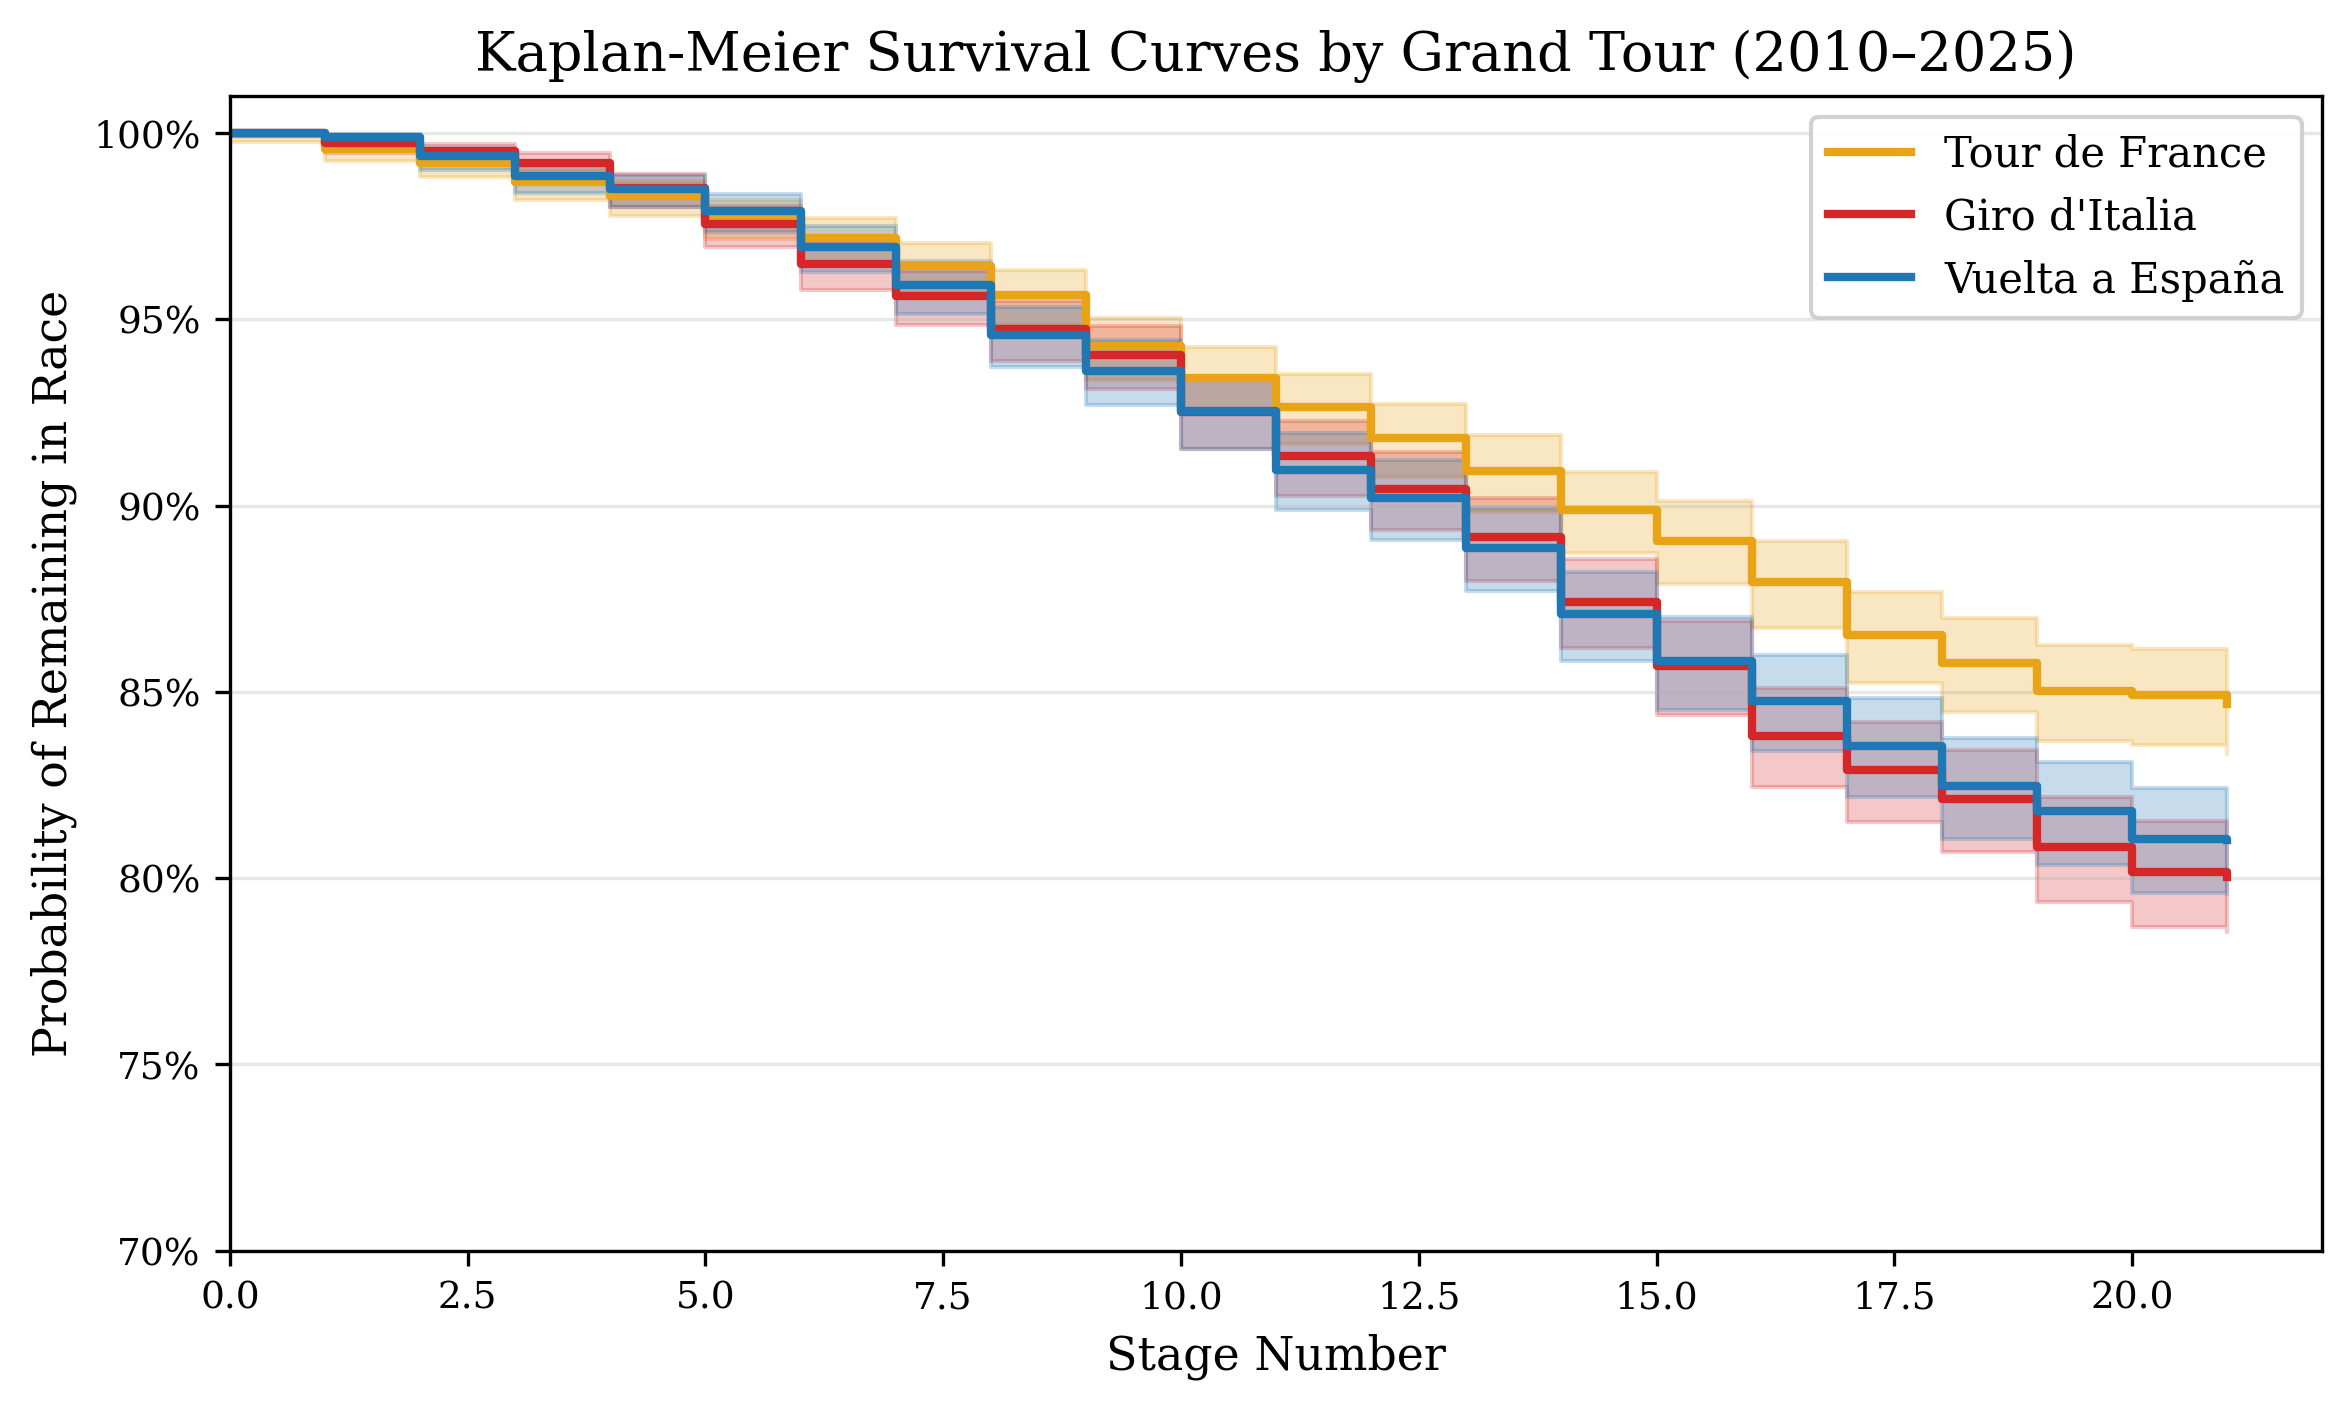
\includegraphics[width=0.6\linewidth]{Afsnit/Billeder/fig1_km_curves.png}
    \caption{Kaplan--Meier survival curves by Grand Tour (2010--2025). The curves show the estimated probability that a rider is still in the race at each stage number, separately for the Tour de France, Giro d'Italia, and Vuelta a Espa\~{n}a. The Tour de France curve lies consistently above the other two, indicating higher survival rates at every stage.}
    \label{fig:km_curves}
\end{figure}

Figure~\ref{fig:dnf_by_year}, already shown in the introduction, adds a temporal dimension: DNF rates fluctuate year to year, but the Tour de France is consistently at or near the bottom. The persistent gap between races points toward a structural difference that the econometric models will capture through the race dummies.